% concatenated from main.tex
\documentclass[a4paper,12pt]{amsart}

\usepackage[
hmarginratio={1:1},     % equal left and right margins
vmarginratio={1:1},     % equal top and bottom margins
textwidth=15cm,        % new text width
textheight=21cm,			% new text height
heightrounded,          % always useful
]{geometry}

\usepackage[utf8]{inputenc}
\usepackage[UKenglish]{babel}
\usepackage{csquotes}
\usepackage{graphicx}
\usepackage[pagebackref=false]{hyperref}
\usepackage{amsfonts, amstext, amsmath, amsthm, amscd, amssymb}
\usepackage[sc]{mathpazo}
\usepackage{mathtools}
\usepackage[dvipsnames]{xcolor}
\usepackage{tikz}
\usetikzlibrary{positioning}
\usepackage{float}
\usepackage{svg}
%\usepackage{svg-extract}
\usepackage[
    backend=biber,
    style=alphabetic,
    sorting=nyt,
	maxnames=10,
    url=false,
    isbn=false,
	doi=false,
]{biblatex}

\hypersetup{
  colorlinks=true,
  linkcolor=black,
  citecolor=black,
  urlcolor=blue,
}

\definecolor{dark-red}{rgb}{0.4,0.15,0.15}
\definecolor{dark-blue}{rgb}{0.15,0.15,0.4}
\definecolor{dark-green}{rgb}{0.15,0.4,0.15}

\addbibresource{bibliography.bib} % path for bibliography
%%%%%%%%%%%%%%%%%%%%%%%%%%%%%%%

\setcounter{tocdepth}{3}
\numberwithin{equation}{section}

\theoremstyle{plain}
\newtheorem{theorem}{Theorem}[section]
\newtheorem{proposition}[theorem]{Proposition}
\newtheorem{lemma}[theorem]{Lemma}
\newtheorem{corollary}[theorem]{Corollary}
\newtheorem{exercise}[theorem]{Exercise}
\newtheorem{conjecture}[theorem]{Conjecture}
\newtheorem{claim}[theorem]{Claim}

\theoremstyle{definition}
\newtheorem{definition}[theorem]{Definition}
\newtheorem{example}[theorem]{Example}
\newtheorem{remark}[theorem]{Remark}
\newtheorem{question}[theorem]{Question}
\newtheorem{answer}[theorem]{Answer}
\newtheorem{convention}[theorem]{Convention}
\newtheorem{problem}[theorem]{Problem}

\newcommand{\variable}{}
\newtheorem*{thm_again*}{Theorem~\ref{\variable}}
\newenvironment{thm_again}[2]
 {
  \renewcommand{\variable}{#1}
  \begin{thm_again*}[#2]
  }
 {
  \end{thm_again*}
  }


\providecommand{\keywords}[1]{\textbf{\textit{Key words and phrases: }} #1}
\providecommand{\subjclass}[1]{\textbf{\textit{2020 Mathematics Subject Classification: }} #1}

%%%%%%%%%%% symbols
\newcommand{\di}{\mathbb{D}}
\newcommand{\s}{\mathbb{S}}
\newcommand{\ZZ}{\mathbb{Z}}
\newcommand{\RR}{\mathbb{R}}
\newcommand{\NN}{\mathbb{N}}
\newcommand{\tr}{\triangleright}
\newcommand{\tl}{\triangleleft}
\renewcommand{\epsilon}{\varepsilon}

\DeclareMathOperator{\rk}{rk}
\newcommand{\retract}{\mathbin{\rotatebox[origin=c]{-45}{$\rightsquigarrow$}}}
%%%%%%%%%%%%% \maketitle
\title{The fundamental quandle of ribbon concordances}
\author{Eva Horvat, Luka Marčič}
\address{University of Ljubljana, Faculty of Education, Kardeljeva plo\v s\v cad 16, 1000 Ljubljana, Slovenia \newline
	University of Ljubljana, Faculty of Mathematics and Physics, Jadranska ulica 19, 1000 Ljubljana, Slovenia}
\email{\href{mailto:eva.horvat@pef.uni-lj.si}{eva.horvat@pef.uni-lj.si}\\
	\href{mailto:luka.marcic@fmf.uni-lj.si}{luka.marcic@fmf.uni-lj.si}}
\subjclass[2020]{57K10, 57K12, 57K45}
\keywords{quandle, fundamental quandle, surface-link, ribbon concordance}
\date{\today}



%%%%%%%%%%%%%%%%%%%%%%%%%%%%%%%%%%%%

\begin{document}

\begin{abstract}
	We describe the fundamental quandle of a properly embedded surface $F$ (possibly with boundary) in $\RR ^{3}\times I$, 
	and derive its presentation in terms of a motion picture diagram or a CH-diagram of $F$. 
	Our study is based on the topological definition of the fundamental quandle. 
	We prove that a ribbon concordance $C$ from a classical knot $K_1$ to $K_0$ gives rise to an injective quandle homomorphism 
	$Q(K_0)\to Q(C)$ and a surjective quandle homomorphism $Q(K_1)\to Q(C)$.
\end{abstract}

\maketitle
	


\section{Introduction}
Quandles are algebraic structures whose axioms are designed to mimic the Reidemeister moves between classical link diagrams. 
Introduced by David Joyce in 1982~\cite{J}, the fundamental quandle provides an almost complete invariant of classical knots. 
From the turn of the century onwards, our knowledge about the algebra of quandles and their numerous applications in knot theory has progressed rapidly,
resulting in a myriad of powerful computable invariants.



The fundamental quandle of a properly embedded codimension 2 submanifold of a connected manifold was topologically defined in~\cite{J} and~\cite{FR}. 
Quandle and biquandle cocycle invariants of closed embedded surfaces in the 4-space have been studied by several authors, see for example~\cite{CKS1}. 
These methods are usually based on some diagram-based algebra without a clear connection with the topological definition. 
In this paper, we try to fill this gap of reasoning by explaining the relationship between the fundamental quandle of an embedded surface $F$ with boundary and the fundamental quandles of its boundary components. 
We construct a presentation of $Q(F)$ from a motion picture diagram of $F$. 
Our procedure also gives a presentation of $Q(F)$ from a CH-diagram or similar (e.g. banded link) diagram. 
Using our construction for a ribbon concordance between two classical knots, we prove a quandle analogue of Gordon's lemma about the knot groups of two ribbon concordant knots:  
\begin{lemma}[\cite{G}]
	\label{lemma:gordon}
	If $C$ is a ribbon concordance from $K_1$ to $K_0$, then $\pi _{1}(K_1)\to \pi _{1}(C)$ is surjective and $\pi _{1}(K_0)\to \pi _{1}(C)$ is injective. 
\end{lemma}
This gives us the main result of this paper.


\begin{theorem}
	\label{thm:ribbon_conc_quandle}
	Let $C\subset \s ^{3}\times I$ be a ribbon concordance from a knot $K_1$ to a knot $K_0$, where $K_{i}\in \s ^{3}\times \{i\}$. 
	Then the induced quandle homomorphism $Q(K_{0})\to Q(C)$ is injective, and $Q(K_{1})\to Q(C)$ is surjective.
\end{theorem}
We conclude the paper with a brief discussion on possible applications and future research directions.



The paper is organized as follows. 
In Section~\ref{sec1}, we review the basics on quandles and their presentations, recall the topological definition of the fundamental quandle of a codimension 2 submanifold and the definition of a ribbon concordance. 
In Section~\ref{sec2}, we discuss fundamental quandles of embedded surfaces. 
Subsection~\ref{subsec2-1}, gives a procedure to obtain the presentation of the fundamental quandle of a properly embedded surface in $\RR ^{4}$ from its motion picture diagram or a CH-diagram.
Subsection~\ref{subsec2-2} then deals with the special case of ribbon concordances, proving theorem~\ref{thm:ribbon_conc_quandle} and ending in a discussion of the results.


























\section{Preliminaries}
\label{sec1}


\subsection{Quandles}
\begin{definition}
	A \textit{quandle} is a set $Q$ with a binary operation $\tr \colon Q\times Q\to Q$ that satisfies the following axioms: 
	\begin{enumerate}
		\item $x\tr x=x$,
		\item the map $R_{y}\colon Q\to Q$, given by $R_{y}(x)=x\tr y$, is a bijection, and
		\item $(x\tr y)\tr z=(x\tr z)\tr (y\tr z)$
	\end{enumerate} for every $x,y,z\in Q$. 
\end{definition}
The second axiom is equivalent to an existence of a second operation defined by $x\tl y=R_{y}^{-1}(x)$, 
such that $(x\tr y)\tl y=x=(x\tl y)\tr y$ for every $x,y\in Q$. 
A \textit{quandle homomorphism} is a function between two quandles $f\colon (Q_{1},\tr _{1})\to (Q_{2},\tr _{2})$ that satisfies the equalities 
$f(x\tr _{1}y)=f(x)\tr _{2}f(y)$ and $f(x \tl_1 y) = f(x) \tl_2 f(x)$ for every $x,y\in Q_1$.




\begin{example}[Conjugation quandle]
	In any group $G$, the operation of conjugation $a\tr b:=b^{-1}ab$ defines a quandle, denoted by $conj(G)$, with
	$a \tl b = b a b^{-1}$.
\end{example}


\begin{definition} 
	Let $Q$ be a set with a binary operation $\tr \colon Q\times Q\to Q$. 
	An equivalence relation $\sim $ on $Q$ is called a $\tr $-\textit{congruence} if $a\sim b\land c\sim d$ implies $a\tr c\sim b\tr d$ for every $a,b,c,d\in Q$. 
\end{definition}
Observe that the induced operation $\tr $ on the quotient $Q/_{\sim }$, given by $[a]\tr [b]=[a\tr b]$, is well-defined iff $\sim $ is a $\tr $-congruence. 
If $(Q,\tr )$ is a quandle and $\sim $ is a $\tr $-congruence and a $\tl $-congruence, then $(Q/_{\sim },\tr )$ is also a quandle.
Note that both congruence conditions are necessary for a rigorous definition~\cite{BT}.




Let $S$ be a set and denote by $F(S)$ the free group over $S$. 
Define operations $\tr$ and $\tl$ on $S \times F(S)$ by $(a,w) \tr (b,z) = (a,w\overline{z}bz)$
and $(a,w) \tl (b,z) = (a,w\overline{z}\overline{b}z)$.
Let an equivalence relation $\sim _{Q}$ on the product $S\times F(S)$ be given by 
$$(a,w_1)\sim _{Q}(b,w_2) \Leftrightarrow a=b\land w_{2}=a^{k}w_1\textrm{ for some }k\in \ZZ \;.$$  
We will denote the quotient set $(S\times F(S))/_{\sim _{Q}}$ by $Q_S$. 
Define an inclusion $\iota \colon S\to Q_{S}$ by $\iota (a)=[a,1]$. 


\begin{lemma} 
	The above relation $\sim _{Q}$ is the smallest $\tr $-congruence and $\tl $-congruence on $S\times F(S)$ for which the quotient set $(S\times F(S))/_{\sim _{Q}}$ with induced operation is a quandle.
	For any group $G$ and any map $f\colon S\to G$, there exists a unique quandle homomorphism $\overline{f}\colon Q_{S}\to conj(G)$ with $\overline{f}\circ \iota =f$.  
\end{lemma}
\begin{proof}
	Suppose that $(a,w_1)\sim _{Q}(a,w_2)$ and $(b,v_1)\sim _{Q}(b,v_2)$ in $S\times F(S)$. 
	It follows that $w_{2}=a^{k}w_{1}$ and $v_{2}=b^{l}v_{1}$ for some $k,l\in \ZZ $, thus $(a,w_i)\tr (b,v_i)=(a,w_{i}\overline{v}_{i}bv_{i})$ and $w_{2}\overline{v}_{2}bv_{2}=a^{k}w_{1}\overline{v}_{1}bv_{1}$. 
	Therefore, $\sim _{Q}$ is a $\tr $-congruence and the operation $\tr $ is well-defined on the equivalence classes.
	Similarly, $\sim _Q$ is a $\tl $-congruence and $\tl$ is well-defined on the equivalence classes.
	For the remainder of the proof, we slightly abuse notation and perform all computations on representatives of the equivalence classes. 


	To verify that $Q_S$ is a quandle, first observe that 
	$$((a,w) \tr (b,z)) \tl (b,z) = (a,w\overline{z}bz) \tl (b,z) = (a, w \overline{z} b z \overline{z} \overline{b} z) = (a,w)$$
	and that, likewise, $((a,w) \tl (b,z)) \tr (b,z) = (a,w)$, showing that the quandle axiom (2) holds.
	Another computation

	\begin{align*}
		\left ((a, w)\tr (c, z)\right )\tr \left ((b, v)\tr (c, z)\right ) &=(a, w\overline{z}cz)\tr (b,v\overline{z}cz) =(a,w\overline{z}cz\overline{z}\overline{c}z\overline{v}bv\overline{z}cz)=\\
		& =(a,w\overline{v}bv\overline{z}cz)=\left ((a,w)\tr (b,v)\right )\tr (c,z)
	\end{align*}
	takes care of the quandle axiom (3). For the quandle axiom (1), compute 
	$$(a,w)\tr (a,w)=(a,w\overline{w}aw)=(a,aw)\sim _{Q}(a,w)$$ 
	and observe that a quotient $(S\times F(S))/_{\sim }$ is a quandle exactly when the congruence $\sim $ contains $\sim _{Q}$. 


	To verify the second claim of the Lemma, let $f$ be any map from the set $S$ to a group $G$ and denote by $\widehat{f}\colon F(S)\to G$ its extension to the free group over $S$. 
	Suppose $\overline{f}\colon Q_{S}\to conj(G)$ is a quandle homomorphism with $\overline{f}\circ \iota =f$.
	Then we have $\overline{f}(a,1)=f(a)$ and
	\begin{align*}
		\overline{f}\left ((a,w)\tr (b,z)\right )&=\overline{f}(a,w\overline{z}bz)\\
		\overline{f}(a,w)\tr \overline{f}(b,z)&=\overline{f}(b,z)^{-1}\overline{f}(a,w)\overline{f}(b,z)
	\end{align*}
	Identifying both expressions for $w=z=1$ yields $\overline{f}(a,b)=f(b)^{-1}f(a)f(b)$, and by extending this over $Q_S$, we obtain $\overline{f}(a,w)=\widehat{f}(\overline{w}aw)$. 
\end{proof}


\begin{definition}
	The quandle $Q_{S}=(S\times F(S))/_{\sim _{Q}}$ is called the \textit{free quandle} over the set $S$.
\end{definition}


The importance of the free quandle comes from the fact that it allows us to define presentations of quandles.


\begin{definition}
	Let $Q$ be a quandle. A \textit{presentation} $\langle X\mid R\rangle$ for $Q$, where $X$ is a set and $R \subset Q_X \times Q_X$,
	is an isomorphism between $Q$ and the quotient quandle $Q_X/{\sim_R}$, where $\sim_R$ is the smallest congruence on $Q_X$ containing $R$. 
	To simplify notations, we will often write $x=y$ instead of $(x,y) \in R$ and $\langle x_1,\ldots, x_m  \mid r_1,\ldots, r_n\rangle$  instead of $\langle \{x_1,\ldots, x_m\}\mid \{r_1,\ldots, r_n\}\rangle$.
	The cardinality of the smallest subset $S \subset Q$ such that $\langle S \rangle = Q$ is called the \textit{rank} of $Q$ and is denoted by $\rk(Q)$.
\end{definition}


Let us recall also the definition of the fundamental quandle of a codimension 2 submanifold of a topological manifold.
From now on, we will denote by $I$ the standard interval $[0,1]$.


\begin{definition}[\cite{FR}]
	Let $L\subset M$ be a properly embedded codimension 2 subma\-ni\-fold of a connected manifold $M$.
	Assume that $L$ is transversely oriented in $M$, denote by $N_{L}$ the normal disk bundle and by $E_{L}=\text{cl}(M-N_{L})$ its exterior. 
	Choose a basepoint $z\in E_L$.
	Define
	$$\Gamma_L := \frac{\mathcal{C}( (I, \{0\}, \{1\}) \to (E_L, \partial N_L, \{z\}))}{\text{homotopy}}\; ,$$
	the space of (continuous) paths from $\partial N_L$ to $z$ modulo homotopies fixing the endpoint $z$ and allowing the initial point to wander freely along $\partial N_L$.
	For any point $p\in \partial N_{L}$, denote by $m_{p}$ the loop in $\partial N_{L}$ based at $p$, which follows around the meridian of $L$ in the positive direction.
	The \textit{fundamental quandle} $Q(L)$ of $L$ is the set $\Gamma _{L}$ together with operation
	$$[\alpha]\tr [\beta] := [\alpha \cdot \overline{\beta }\cdot m_{\beta (0)}\cdot \beta ] \;,$$
	where $\overline{\beta}$ denotes the reversal of the path $\beta$ and $\cdot $ denotes the concatenation of paths.
\end{definition}


Different choices of basepoints give rise to isomorphic quandles.
It is clear from the definition that the fundamental quandle is an invariant up to ambient isotopy.


\begin{example}[Fundamental quandle of a link]
	A presentation of the fundamental quandle of a link $L$ in $\s^{3}$ may be obtained from any diagram of $L$; namely, every arc of the diagram corresponds to a generator and every crossing gives a crossing relation (see Figure~\ref{fig:quandle_crossing_relations}).
\end{example}

   


\begin{figure}[H]
	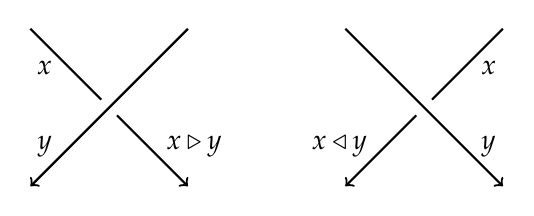
\begin{tikzpicture}
		\draw[black, thick][<-] (-1,-1) -- (1,1);
		\draw[black, thick] (-1,1) -- (-0.1,0.1);
		\draw[black, thick][->] (0.1,-0.1) -- (1,-1);
		\filldraw[black] (-0.6,0.5) node[anchor=east]{$x$};
		\filldraw[black] (-0.6,-0.5) node[anchor=east]{$y$};
		\filldraw[black] (0.6,-0.5) node[anchor=west]{$x\tr y$};


		\draw[black, thick][->] (3,1) -- (5,-1);
		\draw[black, thick][<-] (3,-1) -- (3.9,-0.1);
		\draw[black, thick] (4.1,0.1) -- (5,1);
		\filldraw[black] (4.6,0.5) node[anchor=west]{$x$};
		\filldraw[black] (4.6,-0.5) node[anchor=west]{$y$};
		\filldraw[black] (3.4,-0.5) node[anchor=east]{$x\tl y$};
	\end{tikzpicture}
	\caption{The quandle crossing relations}
	\label{fig:quandle_crossing_relations}
\end{figure}














\subsection{Ribbon concordances}
The study of knot concordances represents a bridge between the classical knot theory and 4-manifold topology.


\begin{definition}
	A \textit{concordance} between two knots $K_{0}$ and $K_{1}$ is the image of a smooth embedding $f\colon (\s^{1}\times I, \s^1 \times \{0\}, \s^1 \times \{1\}) \to (\s^3 \times I, K_0 \times \{0\}, K_1 \times \{1\})$.
	The embedded annulus associated with a concordance will be denoted by $C=f(\s ^{1}\times I)\subset \s ^{3}\times I$. 
	We may assume that the projection $\s ^{3}\times I\to I$ restricted to $C$ is a Morse function, and if it has only critical points of index 0 and 1, $C$ is called a \textit{ribbon concordance} from $K_1$ to $K_0$. 
	A knot $K$ is called \textit{ribbon} if there exists a ribbon concordance from $K$ to the unknot.
\end{definition}




It is clear that concordance gives an equivalence relation on the set of all knots in the 3-sphere. 
Ribbon concordance of knots, however, is not symmetric. 
In his seminal paper~\cite{G}, Gordon introduced notation $K_{1}\geq K_0$ if there exists a ribbon concordance from $K_1$ to $K_0$, and conjectured relation $\geq $ gives a partial order on the set of all knots, which was confirmed forty years later in~\cite{A}.  
 




































\section{The concordance quandle}
\label{sec2}


\subsection{Fundamental quandle of an embedded surface}
\label{subsec2-1}


Knotted surfaces in the 4-space have been studied via several diagrammatic theories~\cite{CS,CKS2}.
One of them, introduced by Roseman~\cite{R}, represents a generic projection of an embedded surface into $\mathbb{R}^{3}$. 
The fundamental quandle of a closed knotted surface given by this presentation was described in~\cite{CKS1}. 
Since we will be interested in the fundamental quandle of a surface with boundary and would like to relate it with the fundamental quandles of its boundary components, a motion picture diagram of a knotted surface will suit our purposes better. 
We will describe the presentation of the fundamental quandle, based on its motion picture. 
This will imply a procedure to obtain a presentation of the fundamental quandle from the banded unlink diagrams or CH-diagrams, introduced by Lomonaco~\cite{L} and further developed by Yoshikawa~\cite{Y}.
%\linebreak


Let $F\subset \RR ^{4}$ be a compact orientable surface. 
Viewing $\RR ^{4}$ as the product $\RR ^{3}\times \RR $, denote by $\pi \colon \RR ^{4}\to \RR $ the projection to the last coordinate. 
$F$ may be isotoped into such position that
\begin{enumerate}
	\item every boundary component of $F$ is contained in a single fibre of $\pi $,
	\item $\pi $ restricts to a Morse function on $F$. 
\end{enumerate}


Every regular fibre of $\pi $ then intersects $F$ in a link, and by drawing the diagrams of subsequent regular fibres we obtain a motion picture diagram of the embedded surface. 
Observe that a finite sequence of stills (classical link diagrams) $\mathcal{M}=(\mathcal{D}_{1},\mathcal{D}_{2},\ldots ,\mathcal{D}_{n})$ is sufficient to fully describe the embedding of $F$.
Figure~\ref{fig2} shows the possible local transformations between two subsequent stills of the motion picture beside plane isotopy.
The first three transformations correspond to the passage over a critical point of the Morse function $\pi$. 
At a critical point of index 0, a 0-handle is added to $F$, which gives birth to a new circle in its boundary link (transformation (i)).
A critical point of index 1 corresponds to a saddle of $F$ where a 1-handle is added, changing the boundary link by connecting two arcs along a band (transformation (ii)). 
A critical point of index 2 corresponds to addition of a 2-handle along an unknotted link component, causing its death (transformation (iii)). 
The local transformations (iv)-(vi) correspond to the Reidemeister moves of the boundary link. 
Transformation (vii) corresponds to the addition of a component of $\partial F$ (that may be knotted), while transformation (viii) corresponds to the ending of $F$ in a (possibly knotted) component of $\partial F$.  


\begin{figure}[H]
	\begin{tikzpicture}
		\matrix
		{
		& \node {
			\begin{tikzpicture}[scale=0.50]
				\draw[black,thick] (0,2.5) node[anchor=center]{(i)};
				\draw (-1.5,-1.5) rectangle (1.5,1.5);
				\draw (-1.5,-6.5) rectangle (1.5,-3.5);
				\draw[white,thick] (0,0) circle (1cm);
				\draw[black, thick][->] (0,-2) -- (0,-3);
				\draw[red,thick] (0,-5) circle (1cm);
			\end{tikzpicture}}; &
		\node {
			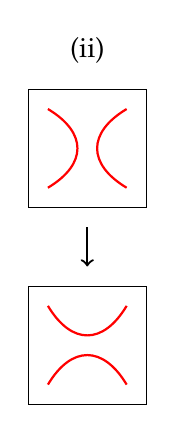
\begin{tikzpicture}[scale=0.50]
				\draw[black,thick] (0,2.5) node[anchor=center]{(ii)};
				\draw (-1.5,-1.5) rectangle (1.5,1.5);
				\draw (-1.5,-6.5) rectangle (1.5,-3.5);
				\draw[red, thick] (-1,1) .. controls (0,0.4) and (0,-0.4) .. (-1,-1) ;
				\draw[red, thick] (1,1) .. controls (0,0.4) and (0,-0.4) .. (1,-1);
				\draw[black, thick][->] (0,-2) -- (0,-3);
				\draw[red, thick] (1,-4) .. controls (0.4,-5) and (-0.4,-5) .. (-1,-4) ;
				\draw[red, thick] (1,-6) .. controls (0.4,-5) and (-0.4,-5) .. (-1,-6);
			\end{tikzpicture}}; & 
		\node {
			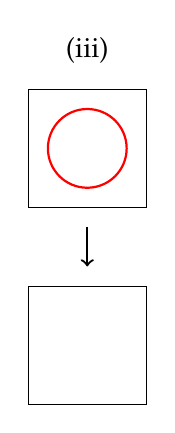
\begin{tikzpicture}[scale=0.50]
				\draw[black,thick] (0,2.5) node[anchor=center]{(iii)};
				\draw (-1.5,-1.5) rectangle (1.5,1.5);
				\draw (-1.5,-6.5) rectangle (1.5,-3.5);
				\draw[red,thick] (0,0) circle (1cm);
				\draw[black, thick][->] (0,-2) -- (0,-3);
				\draw[white,thick] (0,-5) circle (1cm);
			\end{tikzpicture}}; & 
		\node {
			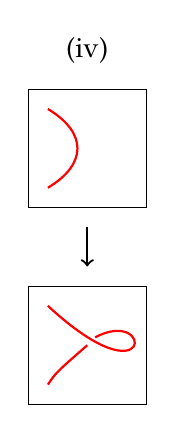
\begin{tikzpicture}[scale=0.50]
				\draw[black,thick] (0,2.5) node[anchor=center]{(iv)};
				\draw (-1.5,-1.5) rectangle (1.5,1.5);
				\draw (-1.5,-6.5) rectangle (1.5,-3.5);
				\draw[red, thick] (-1,1) .. controls (0,0.4) and (0,-0.4) .. (-1,-1) ;
				\draw[black, thick][->] (0,-2) -- (0,-3);
				\draw[red, thick] (-1,-4) .. controls (1.7,-6.5) and (1.7,-4) .. (0.2,-4.8) ;
				\draw[red, thick] (0,-5) .. controls (-0.8,-5.7) .. (-1,-6);
			\end{tikzpicture}}; & 
		\node {
			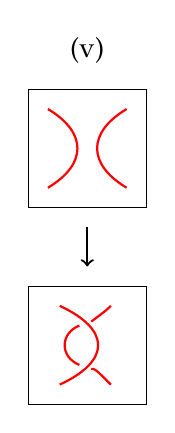
\begin{tikzpicture}[scale=0.50]
				\draw[black,thick] (0,2.5) node[anchor=center]{(v)};
				\draw (-1.5,-1.5) rectangle (1.5,1.5);
				\draw (-1.5,-6.5) rectangle (1.5,-3.5);
				\draw[red, thick] (-1,1) .. controls (0,0.4) and (0,-0.4) .. (-1,-1) ;
				\draw[red, thick] (1,1) .. controls (0,0.4) and (0,-0.4) .. (1,-1);
				\draw[black, thick][->] (0,-2) -- (0,-3);
				\draw[red, thick] (-0.7,-4) .. controls (0.6,-4.6) and (0.6,-5.4) .. (-0.7,-6) ;
				\draw[red, thick] (0.1,-4.4) .. controls (0.5,-4.1) .. (0.6,-4);
				\draw[red, thick] (-0.2,-4.5) .. controls (-0.7,-4.7) and (-0.7,-5.3) .. (-0.2,-5.5);
				\draw[red, thick] (0.1,-5.6) .. controls (0.2,-5.6) .. (0.6,-6);
			\end{tikzpicture}}; & 
		\node {
			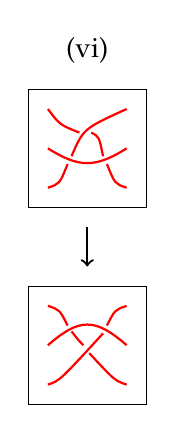
\begin{tikzpicture}[scale=0.50]
				\draw[black,thick] (0,2.5) node[anchor=center]{(vi)};
				\draw (-1.5,-1.5) rectangle (1.5,1.5);
				\draw (-1.5,-6.5) rectangle (1.5,-3.5);
				\draw[red, thick] (-1,-1) .. controls (-0.7,-0.9) .. (-0.5,-0.4) ;
				\draw[red, thick] (-0.4,-0.2) .. controls (-0.1,0.5) .. (1,1);
				\draw[red, thick] (-1,0) .. controls (-0.2,-0.5) and (0.2,-0.5) .. (1,0);
				\draw[red, thick] (-1,1) .. controls (-0.7,0.6) .. (-0.2,0.4);
				\draw[red, thick] (1,-1) .. controls (0.7,-0.9) .. (0.5,-0.4) ;
				\draw[red, thick] (0.4,-0.2) .. controls (0.3,0.3) .. (0.1,0.4) ;
				\draw[black, thick][->] (0,-2) -- (0,-3);
				\draw[red, thick] (-1,-5) .. controls (-0.2,-4.3) and (0.2,-4.3) .. (1,-5);
				\draw[red, thick] (-1,-6) .. controls (-0.7,-5.9) .. (0.4,-4.7) ;
				\draw[red, thick] (0.5,-4.5) .. controls (0.7,-4.1) .. (1,-4);
				\draw[red, thick] (-1,-4) .. controls (-0.7,-4.1) .. (-0.5,-4.5);
				\draw[red,thick] (-0.4,-4.65) .. controls (-0.2,-4.9) ..  (-0.1,-5);
				\draw[red, thick] (1,-6) .. controls (0.7,-5.9) .. (0.05,-5.2) ;
			\end{tikzpicture}}; & 
		\node {
			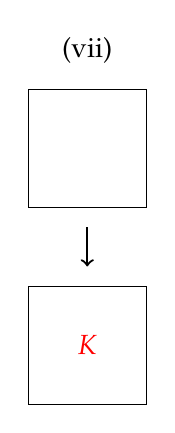
\begin{tikzpicture}[scale=0.50]
				\draw[black,thick] (0,2.5) node[anchor=center]{(vii)};
				\draw (-1.5,-1.5) rectangle (1.5,1.5);
				\draw (-1.5,-6.5) rectangle (1.5,-3.5);
				\draw[white,thick] (0,0) circle (1cm);
				\draw[black, thick][->] (0,-2) -- (0,-3);
				\draw[red,thick] (0,-5) node[anchor=center]{$K$};
			\end{tikzpicture}}; & 
		\node {
			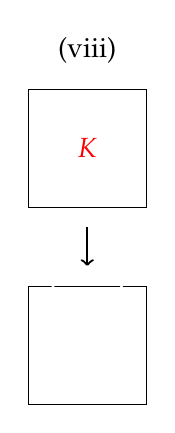
\begin{tikzpicture}[scale=0.50]
				\draw[black,thick] (0,2.5) node[anchor=center]{(viii)};
				\draw (-1.5,-1.5) rectangle (1.5,1.5);
				\draw (-1.5,-6.5) rectangle (1.5,-3.5);
				\draw[red,thick] (0,0) node[anchor=center]{$K$};
				\draw[black, thick][->] (0,-2) -- (0,-3);
				\draw[white,thick] (0,-4) circle (1cm);
			\end{tikzpicture}}; \\
		};
	\end{tikzpicture}
	\caption{Motion picture transformations}
	\label{fig2}
\end{figure}


\begin{lemma} 
	\label{lemma1} 
	Let $L$ be a link in a 3-manifold $M$. 
	Consider $L\times I$ as a properly embedded surface in $M\times I$. 
	The inclusion of pairs $(M\times \{0\},L\times \{0\})\to (M\times I,L\times I)$ induces an isomorphism of the fundamental quandles $Q(L)$ and $Q(L\times I)$. 
\end{lemma}
\begin{proof}
	We identify $(M, L)$ with $(M \times \{0\}, L \times\{0\})$ and thus regard it as a subset of $(M \times I, L \times I)$.
	Let $N_L$ and $N_{L \times I}$ be normal disk bundles of $L$ (in $M$) and $L\times I$ (in $M\times I$), respectively, and
	let $E_L = \text{cl}(M - N_L)$ and $E_{L \times I} = \text{cl}(M \times I - N_{L \times I})$.
	Choose a basepoint $z \in E_L\subset E_{L \times I}$ that defines the fundamental quandles $Q(L)$ and $Q(L \times I)$
	(other choices of basepoint give rise to isomorphic quandles).
	Every path from $\partial N_L$ to $z$ is also a path from $\partial N_{L \times I}$ to $z$, and every homotopy identifying two representatives of an element of $Q(L)$ identifies these representatives in $Q(L\times I)$,
	giving us a well-defined mapping $\iota: Q(L) \to Q(L \times I)$. 
	It follows directly from the definition that $\iota$ is a quandle homomorphism.
	
	Suppose $\alpha$ and $\beta$ are two paths representing elements of $Q(L)$ such that $\iota([\alpha]) = \iota([\beta])$,
	meaning that there exists a homotopy $H\colon I \times I \to E_{L \times I} \subset M \times I$ between $\alpha$ and $\beta$ with $H(\{0\}\times I)\subset \partial N_{L\times I}$ and $H(\{1\}\times I)=\{z\}$. 
	Let $H(t,s) = (H_M(t,s), H_I(t,s))$. Then $\bar{H}: I \times I \to E_L$, defined by $\bar{H}(t,s) = (H_M(t,s), 0)$, 
	is a homotopy between $\alpha$ and $\beta$ in $E_L$ with $\bar{H}(\{0\}\times I)\subset \partial N_{L}$ and $\bar{H}(\{0\}\times I) = \{z\}$. 
	Therefore, $\alpha$ and $\beta$ represent the same element of $Q(L)$, showing that $\iota$ is injective.


	For a path $\gamma(t) = (\gamma_M(t), \gamma_I(t)) \subset E_{L\times I} \subset M \times I$, representing an element of $Q(L \times I)$,
	we can define a homotopy $H_{\gamma}:I \times I \to E_{L\times I}$ from $\gamma$ to a path representing an element in $Q(L)$ by
    $H_{\gamma}(t,s) = \left (\gamma_M(t), (1-s)\gamma_I(t)\right )$,
	showing that $\iota$ is surjective and thus an isomorphism.
\end{proof}






Suppose an embedded surface $F\subset \RR^{4}$ is given by a motion picture diagram $\mathcal{M}=(\mathcal{D}_{1},\mathcal{D}_{2},\ldots ,\mathcal{D}_{n})$. 
The motion picture $\mathcal{M}$ captures the diagrams of the regular fibres $\pi ^{-1}(t_{1}), \pi ^{-1}(t_2), \ldots ,\pi ^{-1}(t_{n})$ of the Morse function $\pi |_{F}\colon F\to \RR $. 
If a neighbourhood $(a,b)$ of the regular value $t_i$ contains no critical values, then $\pi ^{-1}(a,b)\cap F\cong L_{i}\times I$, where $L_i$ is the link in $\RR ^3$ given by the diagram $\mathcal{D}_i$. 
By Lemma~\ref{lemma1}, the fundamental quandle of $\pi ^{-1}(a,b)\cap F$ may then be given by the presentation $\langle X_{i}\mid R_{i}\rangle $ of the classical link quandle $Q(L_i)$, which has a generator for every arc of $\mathcal{D}_i$ and a crossing relation for every crossing of $\mathcal{D}_i$. 


A presentation of the fundamental quandle $Q(F)$ is then obtained from $\mathcal{M}$ by the following procedure: \label{procedure}
\begin{enumerate}
	\item We start by the presentation $\langle X_{1}\mid R_{1}\rangle $ of the fundamental quandle of the link $L_{1}$, represented by the first non-empty motion picture diagram. 
	\item At every transformation of type (i), the presentation $\langle X\mid R\rangle$ transforms to $\langle X\sqcup \{x\}\mid R\rangle $. The new generator $x$ represents the homotopy class of a path from the torus neighbourhood of the newborn circle to the basepoint. 
	\item At every transformation of type (ii), the added 1-handle allows a homotopy between the generators $a$ and $b$, corresponding to the two arcs on the upper picture. A presentation $\langle X\mid R\rangle$ thus transforms to $\langle X\mid R\sqcup \{a=b\}\rangle $.
	\item At a type (iii) transformation, the generator of the fundamental quandle of the dying circle becomes the generator of the fundamental quandle of the whole disc (the 2-handle of $F$), which does not affect the presentation. 
	\item Type (iv), (v) and (vi) transformations do not affect the presentation, as the surface between two links connected by any of these moves is ambient isotopic to a product of one of the links and an interval.
	\item At a type (vii) transformation, the presentation $\langle X\mid R\rangle $ transforms to $\langle X\sqcup X_{K}\mid R\sqcup R_{K}\rangle $, where $\langle X_K\mid R_K\rangle $ denotes the presentation of the fundamental quandle $Q(K)$.
	\item A type (viii) transformation does not affect the presentation.
	\item Once we have applied the above rules to every transformation $\mathcal{D}_{i}\to \mathcal{D}_{i+1}$ for $i=1,2,\ldots ,n-1$, we obtain a presentation for the fundamental quandle $Q(F)$. 
\end{enumerate}


It is a well-known fact that two motion picture diagrams represent ambient isotopic surfaces exactly when they are related by a finite sequence of
movie moves and interchanges of levels of distant critical points. One can easily check that the result of the above construction is
well-defined up to isomorphism with respect to these changes.


The information given by a motion picture diagram of an embedded surface may under certain conditions be given in a more compact form, 
replacing the whole motion picture by a single picture. This idea was first proposed by Fox, and later elaborated by Lomonaco~\cite{L} and Yoshikawa~\cite{Y}. 




\begin{definition} 
	\label{def1} 
	A Morse function $\pi \colon \RR ^{4}\to \RR $ is called a \textit{hyperbolic splitting} of an embedded surface $F\subset \RR ^{4}$ if it satisfies the following conditions:
	\begin{enumerate}
		\item $\pi _{F}$ is also Morse,
		\item all minima of $\pi _{F}$ occur in the level $\pi ^{-1}(-1)$,
		\item all maxima of $\pi _{F}$ occur in the level $\pi ^{-1}(1)$,
		\item all hyperbolic points of $\pi _{F}$ occur in the level $\pi ^{-1}(0)$.
	\end{enumerate}
\end{definition}
Every embedded surface in $\RR ^4$ admits a hyperbolic splitting~\cite{L}. 
We denote by $F_{t}=F\cap \pi ^{-1}(t)$ the $t$-section of the knotted surface, induced by $\pi $, and similarly denote $\RR ^{4}_{t}=\pi ^{-1}(t)$.


A hyperbolic splitting $\pi $ of a knotted surface $F$ may be presented by a marked graph diagram. 
By Definition~\ref{def1}, the 0-section $F_{0}$ defines an embedded 4-valent graph, with vertices corresponding to critical points of index 1 of the Morse function $\pi _{F}$. 
A planar diagram of $F_{0}\subset \RR ^{4}_{0}$ has two kinds of vertices: beside crossing vertices, this diagram contains vertices corresponding to saddles, endowed with markers. 
A marker at a vertex determines the corresponding resolutions below and above the critical point, see Figure~\ref{fig4}. 
We call this diagram a \textit{marked graph diagram} or a \textit{CH-diagram} of $F$ with the hyperbolic splitting $\pi $.
Observe that if $F$ is closed, then for a small $\epsilon >0$ the sections $F_{-\epsilon }$ and $F_{\epsilon }$ are both unlinks. 








\begin{figure}[H]
	\begin{tikzpicture}
		\matrix
		{
		& 
		\node {
			\begin{tikzpicture}[scale=0.5]
				\draw[black,thick] (0,-1.6) node[anchor=north]{$F_{-\epsilon}$};
				\draw[red, thick] (-1,1) .. controls (0,0.4) and (0,-0.4) .. (-1,-1) ;
				\draw[red, thick] (1,1) .. controls (0,0.4) and (0,-0.4) .. (1,-1);
			\end{tikzpicture}}; & 
                     \node {
			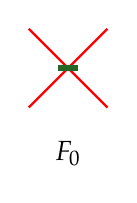
\begin{tikzpicture}[scale=0.5]
				\draw[black,thick] (0,-1.6) node[anchor=north]{$F_{0}$};
				\draw[red, thick] (1,1) -- (-1,-1) ;
				\draw[red, thick] (1,-1) -- (-1,1);
                                          \fill[dark-green,thick] (0.25,0.07) rectangle (-0.25,-0.07);
			\end{tikzpicture}}; & 
	          \node {
			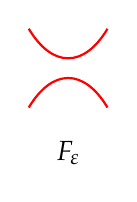
\begin{tikzpicture}[scale=0.5]
				\draw[black,thick] (0,-1.6) node[anchor=north]{$F_{\epsilon }$};
				\draw[red, thick] (1,1) .. controls (0.4,0) and (-0.4,0) .. (-1,1) ;
				\draw[red, thick] (1,-1) .. controls (0.4,0) and (-0.4,0) .. (-1,-1);
			\end{tikzpicture}}; \\
                       };
               \end{tikzpicture}
\caption{The resolutions of a marker below (left) and above the critical point (right)  }
\label{fig4}
\end{figure}


\begin{corollary} 
	Let $\mathcal{D}$ be a marked graph diagram of an embedded surface $F\subset \RR^{4}$ with $m$ markers. 
	Denote by $\mathcal{D}_{-}$ the diagram of the link $F_{-\epsilon }$, obtained by the lower resolution of $\mathcal{D}$ at all markers, and let $\langle X_{\mathcal{D}_{-}}\mid R_{\mathcal{D}_{-}}\rangle $ be the presentation of its fundamental quandle, given by $\mathcal{D}_{-}$. 
	Let $x_{i}$ and $y_i$ denote the two arcs of $\mathcal{D}_{-}$ that meet at the $i$-th marker of $\mathcal{D}$. 
	Then the fundamental quandle $Q(F)$ has a presentation
	\begin{align}
		\label{pres1}
		\left \langle X_{\mathcal{D_{-}}}\mid R_{\mathcal{D}_{-}}\sqcup \cup _{i=1}^{m}\{x_{i}=y_{i}\}\right \rangle \;.
	\end{align}
\end{corollary}
\begin{proof} 
	The marked graph diagram corresponds to a hyperbolic splitting of the embedded surface $F$. 
	Applying the procedure on page \pageref{procedure} to the motion picture of this hyperbolic splitting, we obtain the presentation \eqref{pres1}.
\end{proof}






























\subsection{Fundamental quandle of a ribbon concordance}
\label{subsec2-2}


A ribbon concordance from the knot $K_1$ to $K_0$ is an embedded annulus $C\subset \s ^{3}\times I$ with two knotted boundary components 
$K_{i}=C\cap \left (\s ^{3}\times \{i\}\right )$, whose projection to $I$ is a Morse function without critical points of index 2.
Since the Euler characteristic of $C$ is trivial, the number of 0-handles equals the number of 1-handles. Any ribbon concordance can thus
be represented by a series of ribbon concordances between intermediate knots which have a single 0-handle,
which births a new component, and a single 1-handle, which connects the newborn component to the preceding intermediate knot.
This gives us an inductive approach to dealing with ribbon concordances, having to account for at most one 0-handle and 1-handle pair at a time.


We restate the main theorem of this paper, analogous to lemma~\ref{lemma:gordon}.


\begin{thm_again}{thm:ribbon_conc_quandle}{}
	Let $C\subset \s ^{3}\times I$ be a ribbon concordance from a knot $K_1$ to a knot $K_0$, where $K_{i}\in \s ^{3}\times \{i\}$. 
	Then the induced quandle homomorphism $Q(K_{0})\to Q(C)$ is injective, and $Q(K_{1})\to Q(C)$ is surjective.
\end{thm_again}


To prove the theorem, we will need the following lemma.


\begin{lemma}
	\label{lemma:ribon_conc_quandle}
	Let $C_0\subset \s ^{3}\times [-1, 0]$ be a ribbon concordance from a knot $K_{0}$ to a knot $K_{-1}$,
	and let $C_1 \subset \s^3 \times [0,1]$ be a ribbon concordance from a knot $K_1$ to knot $K_0$, 
	where $K_{i}\in \s ^{3}\times \{i\}$.
	Assume the projection of $C_0$ and $C_1$ to $[-1,1]$ is a Morse function and that the projection of $C_1$ to $[0,1]$ has a single critical point of index 0 and a single
	critical point of index 1. Let $C = C_0 \cup C_1$ be a ribbon concordance from knot $K_1$ to knot $K_{-1}$.
	Then the quandle homomorphism $\iota \colon Q(C_0)\to Q(C)$, induced by inclusion, is injective.
\end{lemma}
\begin{proof} 
	We begin by establishing some notation. 
	We may assume that the ribbon concordance $C_1$ ends at the exact moment when the 1-handle has been attached (it doesn't meaningfully change after that).
	Then $C_1$ consists of a part that is ambient isotopic to $K_0 \times I$ (so that is what we will call it and regard it as), a disk $D$
	and a band $B$, connecting $K_0 \times I$ to $D$ (see Figure~\ref{fig:ribbon_conc} for an example). Define normal disk bundles
	$N_{C_0} \subset \s^3 \times [-1,0]$ and $N_C \subset \s^3 \times [-1,1]$ about $C_0$ and $C$, respectively,
	along with their respective exteriors $E_{C_0} \subset \s^3 \times [-1,0]$ and $E_C \subset \s^3 \times [-1,1]$.
	Notice $N_{C_0}  \subset N_C$ and $E_{C_0} \subset E_C$.
	Lastly, choose a basepoint $z \in E_{C_0}$ for which we define fundamental quandles $Q(C_0)$ and $Q(C)$.


	We can regard both disk $D$ and band $B$ as the product $I \times I$. For clarity's sake we write $D = I_D \times I_D$ and $B = I_B \times I_B$, where $B$ is attached
	to some arc of $K_0 \times {1}$ {along} $I_B \times \{0\}$, and is attached to $I_D \times \{0\} \subset D$ {along} $I_B \times \{1\}$ in the natural way.
	We have a series of strong deformation retractions
	{ \small
	$$C_1 = (K_0 \times I) \cup B \cup D \overset{I_D \times I_D \retract I_D \times \{0\}}{\longrightarrow} (K_0 \times I) \cup B 
	\overset{I_B \times I_B \retract I_B \times \{0\}}{\longrightarrow} K_0 \times I
	\overset{K_0 \times I \retract K_0 \times \{0\}}{\longrightarrow} K_0$$
	}
	which, in turn, give us a strong deformation retraction $R \colon N_C \times I \to N_{C_0}$.


	Since multiple copies of the interval $I$ with distinct meanings will appear from now on, we index them by the variable we use for them; $t$ for $I_t$, $s$ for $I_s$ and $r$ for $I_r$.
	Let $[\alpha], [\beta] \in Q(C_0)$ be such that $\iota([\alpha]) = \iota([\beta]) \in Q(C)$. By definition, $\alpha$ and $\beta$ are paths 
	$(I_t, \{0\}_t, \{1\}_t) \to (E_{C_0}, \partial N_{C_0}, \{z\})$, and we have a homotopy $H\colon I_t \times I_s \to E_{C}$ such that $H(t,0) = \alpha(t)$, $H(t,1) = \beta(t)$,
	$H(0,s) \in \partial N_C$ and $H(1,s) = z$.
	Fixing $t=0$, $H(0,s)$ defines a path in $\partial N_{C}$ from $\alpha(0)$ to $\beta(0)$. The retraction $R \colon N_C \times I_r \to N_{C_0}$ then defines 
	a homotopy $\widetilde{H}_0\colon \{0\}_t \times I_s \times I_r \to \partial N_{C} \subset E_C$,
	where $\widetilde{H}_0(0, s, 0) =  H(0,s)$ and $\widetilde{H}_0(0,s,1)$ is some path in $\partial N_{C_0}$ from $\alpha(0)$ to $\beta(0)$.
	Note that, a priori, the retraction $R$ need not map $H(0,s)$ entirely to $\partial N_C$ for every $r$; it may happen that $R(H(0,s),r) \in \text{int}(N_C)$ for some $s$ and $r$!
	It is clear from the relatively simple definition of $R$ that this happens exactly when $H(0,s)$ moves over a part of $\partial N_C$ defined by the boundary of the disk bundle of some point in $(0,1)_D \times \{1\}_D$.
	To avoid this, we can compose $R$ with a homotopy that first moves $H(0,s)$ along $\partial N_C$ 
	into a favourable position (outside the disk bundles of points in $(0,1)_D \times \{1\}_D$) where this doesn't happen, thus obtaining $\widetilde{H}_0$ as desired
	(see figure~\ref{fig:conc_nbh}).
	Define also $\widetilde{H}_0(1,s,r) = z$.
	Now, since $(I_t \times I_s, \{0,1\}_t \times I_s )$ is a CW-pair, it has the homotopy extension property. 
	Thus, the homotopy $\widetilde{H}_0$ can be
	extended to a homotopy $\widetilde{H}\colon I_t \times I_s \times I_r \to E_C$ such that 
	$\widetilde{H}(0,s,r) = \widetilde{H}_0(0,s,r) \in  \partial N_C, \widetilde{H}(1,s,r) = \widehat{H}_0(1,s,r) = z$ and $\widetilde{H}(t,s,0) = H(t,s)$.
	As such, $\widetilde{H}(t,s,1)$ is then a homotopy in $E_C$ between $\alpha$ and $\beta$ such that $\widetilde{H}(0,s,1) \subset \partial N_{C_0}$ and $\widetilde{H}(1,s,1) = z$.
	Projecting $\widetilde{H}(t,s,1)$ onto $E_{C_0}$ then gives us the desired homotopy between $\alpha$ and $\beta$,
	showing that $[\alpha] = [\beta]$ as elements of $Q(C_0)$.
\end{proof}


\begin{figure}[ht]
	\centering
	%\includesvg[width =0.6\textwidth]{svg-inkscape/ribbon_concordance.svg}
	\includegraphics[page=2, width =0.6\textwidth]{figures/ribbon_concordance.pdf}
	\caption{Example of a ribbon concordance with one critical point of index 0 and 1 each.}
	\label{fig:ribbon_conc}
\end{figure}


\begin{figure}[ht]
	\centering
	\hspace{1cm}
	%\includesvg[width =0.45\textwidth]{svg-inkscape/concordance_neighbourhood.svg}
	\includegraphics[page=2, width =0.45\textwidth]{figures/concordance_neighbourhood.pdf}
	\caption{Fixing $H(0,s)$ so that it doesn't pass $N_C((0,1)_D \times \{1\}_D)$.}
	\label{fig:conc_nbh}
\end{figure}



We can now prove the theorem.
\begin{proof}[Proof of theorem~\ref{thm:ribbon_conc_quandle}]
	The projection of $C$ to $I$ is a Morse function. Since the Euler characteristic of $C$ is trivial ($C$ is an annulus), the number of
	0-handles equals the number of 1-handles.
	By Morse theory, we can assume that the $k$ critical points of index $0$ are mapped to values
	$$\frac{1}{2k +1}, \frac{3}{2k+1}, \dots, \frac{2i-1}{2k+1}, \dots, \frac{2k-1}{2k+1}\, ,$$
	while the $k$ critical points of index $1$ are mapped to values
	$$\frac{2}{2k+1}, \frac{4}{2k+1}, \dots, \frac{2i}{2k+1}, \dots, \frac{2k}{2k+1}\,.$$
	Identifying $\s^3 \backslash \{\ast\}$ with $\RR^3$, we can define the motion picture diagram
	$$\mathcal{M} = \{\mathcal{D}_0, \mathcal{D}_{1}, \dots, \mathcal{D}_{i}, \dots, \mathcal{D}_{2k}, \mathcal{D}_{2k+1}\}\, ,$$
	where the diagram $\mathcal{D}_{i}$ represents the link 
	$K_{i} := C \cap (\s^3 \times \{\tfrac{i + \epsilon}{2k+1}\})$ for $i \in \{1, \dots, 2k\}$,
	$0 < \epsilon <  1$, while the diagrams $\mathcal{D}_0$ and $\mathcal{D}_{2k+1}$ represent $K_0$ and $K_1$, respectively.
	
	\textbf{$\bullet$ monomorphism:}
	We can inductively construct a presentation for $Q(C)$ by the procedure, described on page~\pageref{procedure}.
	Define ribbon concordances $C_i := C \cap (\s^3 \times [0, \tfrac{i+\epsilon}{2k+1}])$
	and their fundamental quandles $Q_{i} := Q(C_i)$ for $i\in  \{0,\dots, 2k\}$. Notice that $Q_0 \cong Q(K_0)$ and $Q_{2k} \cong Q(C)$.
	To get a presentation of $Q_{2i}$ from $Q_{2i-2}$, we extend $C_{2i-2}$ to $C_{2i}$ by adding a 0-handle and then a 1-handle. By lemma~\ref{lemma:ribon_conc_quandle},
	{the quandle homomorphism $Q_{2i-2} \hookrightarrow Q_{2i}$ induced by inclusion is injective.}
	Combining {these}, we get
	$$Q(K_0) \cong Q_0 \hookrightarrow Q_{2} \hookrightarrow Q_{4} \hookrightarrow \dots \hookrightarrow Q_{2k-2} \hookrightarrow Q_{2k} \cong Q(C)$$
	and therefore $Q(K_0) \hookrightarrow Q(C)$.


	\textbf{$\bullet$ epimorphism:}
	We can also construct a presentation for $Q(C)$ by looking at the motion picture backwards, as a cobordism from $K_1$ to $K_0$ with critical points of index 1 and 2.
	Define the fundamental quandles $Q'_{i} := Q(C \cap (\s^3 \times [\tfrac{i - \epsilon}{2k+1},1]))$ for $i \in \{1, \dots, 2k+1\}$.
	Notice that $Q'_{2k+1} \cong Q(K_1)$ and $Q'_1 \cong Q(C)$.
	To get a presentation of $Q'_{2i}$ from $Q'_{2i+1}$, we add a relation (attach a 1-handle).
	To get a presentation of $Q'_{2i-1}$ from $Q'_{2i}$, we need do nothing (attach a 2-handle).
	As such, we have a surjective quotient homomorphism $Q'_{2i+1} \twoheadrightarrow Q'_{2i-1}$.
	Combining these, we get
	$$ Q(K_1) \cong Q'_{2k+1} \twoheadrightarrow Q'_{2k-1} \twoheadrightarrow \dots \twoheadrightarrow Q'_5 \twoheadrightarrow Q'_{3} \twoheadrightarrow Q'_{1} \cong Q(C)$$
	and therefore $Q(K_1) \twoheadrightarrow Q(C)$.
\end{proof}


Theorem~\ref{thm:ribbon_conc_quandle} provides, in theory, powerful obstructions to ribbon concordances between knots based on their fundamental quandles.
In practice, useful (minimal) presentations of fundamental quandles are often excruciatingly difficult to obtain and work with.
There are some families of knots where such presentations can be obtained quite easily: for example knots that can be represented
as closures of braids with two strands, which includes $T(p,2)$ torus knots, will have fundamental quandles of rank two (with the sole exception of the unknot).
More generally, any knot that can be represented as a closure of a braid with $q$ strands will have a fundamental quandle of rank $\leq q$.
This includes torus knots $T(p,q)$ for coprime integers $1 < q< p$, as they can be represented by diagrams shown on figure~\ref{fig:torus_knot}.
It is, however, difficult to show that quandle presentations obtained from such diagrams are minimal in terms of number of generators.


\begin{figure}[ht]
	\centering
	%\includesvg[width =\textwidth]{svg-inkscape/torus_knot.svg}
	\includegraphics[page=2, width = \textwidth]{figures/torus_knot.pdf}
	\caption{Diagram of $T(p,q)$ with marked quandle generators.}
	\label{fig:torus_knot}
\end{figure}


It would be interesting to see how invariants defined from the fundamental quandle of a knot, such as colouring invariants and
quandle cocycle invariants, interact with ribbon concordances. They could possibly provide more computable obstructions to ribbon
concordances between knots. Such is the case for surface knots, where one can directly relate the cocycle invariants of 
ribbon concordant surface-knots, as was shown in~\cite{CKS3}. The proof used there, however, does not
directly translate to the theory of ribbon concordances between classical knots; for a ribbon concordance from $K_1$ to $K_0$, a quandle colouring
of $K_1$ does not necessarily induce a quandle colouring of $K_0$. As such, a more subtle approach would be needed.
Another possible continuation of this study would be looking into how different quandle-like objects, such as racks, kei and biquandles, behave 
under ribbon concordances.



\section*{Acknowledgements}
Both authors are supported by the Slovenian Research Agency grant P1-0292.



\printbibliography
%\begin{thebibliography}{1}
%
%% \bibitem{} , {\em }, , / (), --.
%
%\bibitem{A} I. Agol, {\em Ribbon concordance of knots is a partial ordering}, Communications of the American Mathematical Society \textbf{2}, 374--379, 2022.
%
%\bibitem{BT} W. Burrows, C. Tuffley, {\em The rack congruence condition and half congruences in racks}, Journal of Knot Theory and Its Ramifications, 2025.
%
%\bibitem{CKS1} J. S. Carter, S. Kamada, M. Saito, {\em Diagrammatic computations for quandles and cocycle knot invariants}, Contemp. Math., 318, 51--74, 2003.
%
%\bibitem{CKS3} J. S. Carter, S. Kamada, M. Saito, {\em Ribbon concordance of surface-knots via quandle cocycle invariants}, Journal of the Australian Mathematical Society \textbf{80}, 131 -- 147, 2003.
%
%\bibitem{CKS2} J. S. Carter, S. Kamada, M. Saito, {\em Surfaces in 4-space}, vol. 142 of Encyclopaedia of Mathematical Sciences. Springer-Verlag, Berlin, 2004.
%
%\bibitem{CS} J. S. Carter and M. Saito, {\em Knotted surfaces and their diagrams}, vol 55 of Math. Surveys and Monographs, American Mathematical Society, 1998.
%
%\bibitem{FR} R. Fenn, C. Rourke, {\em Racks and links in codimension two}, J.~Knot Theory Ramifications \textbf{1} 343--406, 1992.
%
%\bibitem{G} C. McA. Gordon, {\em Ribbon concordance of knots in the 3-sphere}, Mathematische Annalen \textbf{257}, 157--170, 1981.
%
%\bibitem{J} D. Joyce, {\em A classifying invariant of knots, the knot quandle}, Journal of Pure and Applied Algebra \textbf{23}, 37--65, 1982
%
%\bibitem{L} S. J. Lomonaco, {\em The homotopy groups of knots I. How to compute the algebraic 2-type}, Pacific Journal of Mathematics \textbf{95}, No. 2, 349--390, 1981. 
%
%\bibitem{R}  D. Roseman, {\em Reidemeister-type moves for surfaces in four-dimensional space}, Knot Theory, Banach Center Publications, Vol. 42, 347–380, 1998.
%
%\bibitem{Y} K. Yoshikawa, {\em An enumeration of surfaces in four-space}, Osaka J. Math., 31, 497--522, 1994.
%
%\end{thebibliography}

\end{document}


